%%%%%%%%%%%%%%%%%%%%%%%%%%%%%

% Configuracion del documento
\documentclass[hidelinks,12pt]{article}
\usepackage[T1]{fontenc}
\usepackage[utf8]{inputenc}
\usepackage[spanish,es-tabla]{babel}
\parindent=0cm %modificar tamaño de sangria
\usepackage{amsmath}
\usepackage{amssymb,amsfonts,latexsym,cancel}
\usepackage{graphicx, xcolor}
\usepackage{epstopdf}
\usepackage{float}
\usepackage{subfigure}
\usepackage{array}
\usepackage{longtable}
\newcolumntype{E}{>{$}c<{$}}
\setcounter{MaxMatrixCols}{40}
\usepackage{bm}
\usepackage[nottoc]{tocbibind}

\usepackage{ragged2e}
\setlength{\parindent}{1.5cm}
\setlength{\parskip}{0.2cm}
\usepackage{tasks}
\settasks{label-format={\color{green!70!black}\large\bfseries}, label-align=center, label-offset={10mm}, label-width={10mm}, item-indent={5mm}, item-format={\scshape\small}, column-sep={3mm}, after-item-skip=-1mm, after-skip={3mm}
}
\usepackage[driverfallback=hypertex]{hyperref}

%%%%%%%%%%%%%%%%%%%%%%%%%%%%%%%%%%%%%%
%% Paquetes o configuración nueva
%---->%%%%%%%%%%%%%%%%%%%%%%%%%%%%%%%%
\usepackage[lmargin=2.5cm,rmargin=2cm,top=3.2cm,bottom=5.3cm,head=1.3cm]{geometry}
\setlength\footskip{1cm}

\usepackage{fancyhdr}

\pagestyle{fancy}
\fancyhead{} % Eliminar definiciones previas en la parte superior
\definecolor{heading}{rgb}{1,0,0}

\renewcommand{\headrulewidth}{3pt} % Esconder linea negra del encabezado
\definecolor{ured}{RGB}{128,0,0}
\renewcommand{\headrule}{\hbox to\headwidth{%
  \color{ured}\leaders\hrule height \headrulewidth\hfill}}

\fancyhead[C]{
\includegraphics[width=17.5cm,height=3.3cm]{assets/images/00_HEADER2}}

\fancyfoot[l]{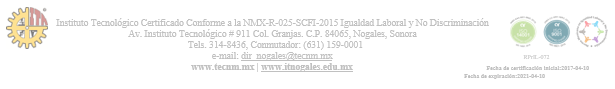
\includegraphics[width=17.01cm,height=2.46cm]{assets/images/00_FOOTER}}

%\fancyfoot[R]{\thepage}

\begin{document}

% ======================%
% ====== PORTADA ====== %
% ======================%
\newgeometry{lmargin=2.5cm,rmargin=2cm,top=1cm,bottom=1cm}
\begin{titlepage}
\begin{center}
\begin{figure}
	
\includegraphics[width=17.5cm,height=3.3cm]{assets/images/00_HEADER}
\end{figure}
\vspace*{1\baselineskip}
{
	\bf\fontsize{13.5}{0}{INSTITUTO TECNOLÓGICO DE NOGALES}\\
}
%\large{\textbf{}}\\
\vspace*{1\baselineskip}
\large{\textbf{MATERIA}}\\
\vspace*{1\baselineskip}
\large{\textbf{TEMA}}\\
\large{\textbf{TEMA}}\\
\vspace*{1\baselineskip}
\large{\textbf{EQUIPO \#X}}\\
NOMBRE 1\\
NOMBRE 2\\
NOMBRE 3\\
\vspace*{1\baselineskip}
\large{\textbf{Número de control}}\\
NO. CONTROL 1\\
NO. CONTROL 2\\
NO. CONTROL 3\\
\vspace*{1\baselineskip}
\large{\textbf{ING. MECATRONICA}}\\
\vspace*{8\baselineskip}
\large{
\textbf{H. Nogales, Sonora \hfill [MES-2020]}}\\
\vspace*{1\baselineskip}
\begin{figure}[h!]
	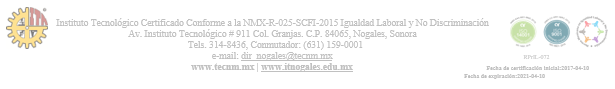
\includegraphics[width=17.01cm,height=2.46cm]{assets/images/00_FOOTER}
\end{figure}
\end{center}
\end{titlepage}
\restoregeometry

% ======================%
% ======= INDICE =======%
% ======================%
\vspace{3cm}
\  \\
\
\tableofcontents
\newpage

% ==============================%
% ======= INDICE FIGURAS =======%
% ==============================%
% \listoffigures
% \newpage


% =========================%
% ======= CONTENIDO =======%
% =========================%
\section{Introduccion}
Esta es la introduccion
\newpage


\section{Desarrollo}
Este es el desarrollo
\newpage


\section{Conclusion}
Esta es la conclucion
\newpage

% ===========================%
% ======= REFERENCIAS =======%
% ===========================%

% \begin{thebibliography}{100}

% \bibitem{ref1}
% \url{http://www.informaticamoderna.com/Supresor_picos.htm }
% \emph{El supresor de picos y la barra multicontacto}
% \end{thebibliography}

\end{document}
